\section{Go}\label{sec:tech:go}
Go ist eine für Systemprogrammierung (Dienste, Treiber, etc.) ausgelegte Programmiersprache mit kurzer und prägnanter Syntax. Entwickelt wurde die Sprache unteranderem von Robert Griesemer, Rob Pike und Ken Thompson (vgl. \cite{go:wiki}). Go bietet unteranderem automatische Speicherverwaltung, Typsicherheit, Closures, effiziente Nebenläufigkeitsmechanismen (goroutines). Go wird vor allem als serverseitige Programmiersprache für Webanwendungen und Microservices in Verbindung mit Virtualisierungsumgebungen wie Docker  eingesetzt.
\begin{wrapfigure}{r}{0.35\textwidth}
    \centering
    \includesvg[width=0.19\textwidth]{MJ/assets/Go_Logo_Blue.svg}
    \caption{Go Logo (vgl. \cite{GoLogoBlue})}
\end{wrapfigure}
Die Implementierung des Teilbereichs zur zentralen Schnittstelle des Systems (Kapitel \ref{ch-implementation}) des vorliegenden Projektes wurde ausschließlich in Go verfasst. Da Go eine relativ moderne Programmiersprache ist, und demnach weniger damit vertraut sind, werden in den folgenden Absätzen die wichtigsten Konzepte der Sprache anhand von Beispielen erklärt. Da sich speziell die Konzepte zum Thema Nebenläufigkeit in Go, doch sehr stark von beispielsweise Java oder ähnlichen Sprachen unterscheiden, werden diese hier etwas genauer erklärt um essentielle Teile der Implementierung zu verdeutlichen.\bigskip

\noindent
\textbf{Kurz zum Hintergrund:} \textit{Wieso Go? Wieso nicht Java oder Python?}\\
Der Hauptgrund für den Einsatz von Go als Programmiersprache eines beachtlichen Projektes, wie einer Diplomarbeit, war der Lernfaktor. Nach dem Einsatz von Go im Rahmen einiger privater Projekte, war Ich bereits mit der Sprache sowie dessen Eigenheiten vertraut. Die Alleinstellungsmerkmale (Goroutines, Concurrency, Channels) der Sprache und deren Ausführung, sind zum Großteil sehr elegant und clever gelöst. Vor allem der fehlende Overhead, verglichen mit Technologien wie Java, mit denen man ohne IDE und mehreren Frameworks nicht weit kommt, erleichtert den Entwicklungsprozess sehr. Die kompakte Syntax in Kombination mit statischen Typen ist ebenfalls sehr gut gelöst. Die erwähnten Mechanismen wie goroutines in Kombination mit Channels welche auf den ersten Blick mit Threads vergleichbar sind, erlauben es, anders über Probleme zum Thema Nebenläufigkeit nachzudenken und Lösungen zu finden, welche man mit herkömmlichen Technologien möglicherweise nicht erreicht hätte.\\
Zusammenfassend lässt sich sagen, dass die Beliebtheit von Go in Entwicklerkreisen definitiv gerechtfertigt ist.\bigskip 

\noindent
In den folgenden Abschnitten werden kurz die für die Implementierung relevanten Features der Sprache erklärt.
% \subsection{Relevante Features}
\subsection{Strukturen und Sichtbarkeit}
Ein \mono{struct} ist eine Sammlung von Datenfeldern, an welches Methoden angehängt werden können (vgl. \cite{go:spec:structs}). Structs sind vergleichbar mit Klassen in herkömmlichen Programmiersprachen wie Java. An ein solches Struct können Methoden angehängt werden, welche den Zustand der sich im struct befindlichen Datenfelder verändern.\bigskip

\noindent
\newpage
Hier ein Beispiel wie Structs in Kombination mit Methoden eingesetzt werden um Getter und Setter eines User-Objektes abzubilden. 
{\ColorfulCodeDisclaimer}
% \begin{minipage}[c]{\linewidth}
\begin{lstlisting}[style=goMono,caption={Struct in Kombination mit Methoden}]
type User struct {
    id        int    %\color{magenta}(1)%     
    Firstname string  
    Lastname  string 
}

func %\color{magenta}(2)% (u User) GetId() int {
    return u.id
}

func %\color{magenta}(3)% (u *User) SetId(id int) {
    u.id = id
}
\end{lstlisting}
% \end{minipage}
Im obigen Beispiel werden bereits einige Eigenheiten von Go demonstriert.\bigskip

\noindent
Go regelt die Sichtbarkeit von Variablen, Konstanten, Funktionen und Strukturen anders, manche meinen sogar eleganter, als beispielsweise Java. Es wird nicht jedes Element (Variablen, Funktionen, etc.) einzeln mit einem Sichtbarkeitsmodifizierer wie \mono{public} oder \mono{private} ausgestattet, sondern die Schreibweise des jeweiligen Elements wird beachtet. Elemente, welche mit kleinem Anfangsbuchstaben beginnen sind nur innerhalb der jeweiligen Übersetzungseinheit sichtbar (also innerhalb des \frqq{}\mono{package xyz}\flqq{}). Elemente, die mit großem Anfangsbuchstaben beginnen sind öffentlich sichtbar.\bigskip

\noindent
Mit diesem Hintergrundwissen ausgestattet sollte auch sofort ersichtlich sein wieso für das Attribut \mono{\color{magenta}(1)} \mono{id} Getter und Setter definiert werden müssen. Nun zu \mono{\color{magenta}(2)} und \mono{\color{magenta}(3)}. Dies sind Bespiele für Methoden, also Funktionen die an eine Struktur angehängt wurden und auf die inneren Attribute lesend oder schreibend, zugreifen können. In letzterer Aussage liegt auch gleich der Unterschied zwischen den beiden hervorgehobenen Punkten: lesend, technisch korrekt formuliert \textit{Call-By-Value} und schreibend, also \textit{Call-By-Reference}.  

\newpage
\subsubsection{Struct-Tags}
Datenfelder einer Struktur können mit Attributen ausgezeichnet werden, die von Bibliotheken und Frameworks genutzt werden um beispielweise den JSON-Namen eines Attributes zu definieren (vgl. \cite{go:spec:structs}).\\
Hier ein Bespiel wie \frqq{}struct-tags\flqq{} in Go eingesetzt werden um ein Objekt zu serialisieren.
\begin{lstlisting}[style=goRaw,caption={\centering Objekt \textit{User}, welches mit struct-tags annotiert wurde um die JSON-Serialisierung zu konfigurieren.}]
type User struct {
    ID        int     `json:"-"`
    Firstname string  `json:"my_firstname"`
    Lastname  string  `json:"my_lastname"`
    Skills    []Skill `json:"my_skills"`
}
\end{lstlisting}
Das obige Beispiel demonstriert, wie \frqq{}struct-tags\flqq{} also herkömmliche doppelte Hochkommas (\mono{"}) bzw. rückwärts geneigte Hochkommas (\mono{\`{}}) (engl. \textit{backticks}), dazu verwendet werden, Datenfelder im Struct mit Attributen zu versehen, welche in diesem Fall von dem JSON-Parser in der Standardbibliothek (über ein Reflection Interface im \frqq{}\mono{reflect}\flqq{} package) eingelesen werden. Eine mit \frqq{}\mono{json.Marshal}\frqq{} (vgl. \cite{go:pkg:json:marshal}) serialisierte Instanz der obigen Struktur könnte folgendermaßen aussehen:\\
\verb|{"my_firstname": "Max", "my_lastname": "Mustermann", "my_skills": ["mustern"]}|.\\
Wie erwartet werden die konfigurierten Felder richtig benannt, die \frqq{}Skills\frqq{} auch korrekt als JSON-Array serialisiert und das \mono{ID}-Feld wurde ignoriert da es in der Definition mit \verb|json:"-"| annotiert wurde. 

\subsection{Aufzählungen}
Aufzählungen, auch bekannt unter Enumerationen gruppieren ähnliche Attribute. Aufzählungen in Go funktionieren anders als in Java oder vergleichbaren Sprachen. In Go wird \mono{iota} verwendet um fortlaufende Aufzählungen zu generieren. \mono{iota} ist ein Zähler der standardmäßig bei 0 beginnt und nach jedem Element in der Aufzählung um 1 erhöht wird. Dieses Verhalten kann durch verschiedene Ausdrücke konfiguriert werden. Dieser Zähler wird nach jeder Aufzählung wieder auf 0 zurückgesetzt. Folgendes Beispiel, das eine Aufzählung von verschiedenen Automarken definiert, veranschaulicht das beschriebene Konzept.
\begin{lstlisting}[style=goMono,caption={Aufzählung von Automarken},label={lst:tech:go:enum:ex1}]
const (
    Jeep = iota + 1 %\color{magenta}(1)%
    _
    Audi     
    Mercedes
    Volkswagen
    LandRover
)
\end{lstlisting}
Der Vollständigkeit halber befindet sich im Anhang (siehe Abschnitt \ref{sec:apdx:extendedcode}) der vollständige Go-Code, welcher die im obigen Listing angegebene Ausgabe erzeugt.\\
Hier erfolgt nun eine kurze Erklärung, wie der obige Ausschnitt zu verstehen ist. Die mit \mono{\color{magenta}(1)} markierte Zeile im Listing ist die eigentliche Aufzählung. Hier wird \mono{iota}, eine ganzzahlige Konstante, verwendet um den sich innerhalb der Aufzählung \mono{( ... )} befindlichen Namen einen Wert zuzuordnen. Da \mono{\color{magenta}(1)} die einzige Zuweisung ist, wird diese für die restlichen Namen wiederholt. Nun wird \mono{iota} für jedes Auto um 1 erhöht sodass den Autos schlussendlich folgende Konstanten zugewiesen werden: \mono{Jeep}=1, \mono{Audi}=3, \mono{Mercedes}=4, \mono{Volkswagen}=5, \mono{LandRover}=6. Der \mono{\_} Indentifier steht immer für einen Namen der ignoriert wird, darum wird \mono{Audi} auch der Wert 3, statt 2, zugeordnet.

\subsection{Concurrency Patterns in Go}
\begin{tcolorbox}
\centering\textit{%
\frqq{}Do not communicate by sharing memory; instead, share memory by communicating.\flqq \cite{go:proverbs:concurrency} }
\end{tcolorbox}\bigskip
% https://go.dev/blog/codelab-share
\noindent
Concurrency, dt. Gleichzeitigkeit, also Prozesse welche gleichzeitig ausgeführt werden, sollten in Go dem oben genannten Ideal folgen: Kommunikation zwischen gleichzeitig ablaufenden Prozessen mittels Nachrichtenaustausch. Damit ist gemeint, dass Prozesse die gleichzeitig ablaufen (goroutines), sich über eine gemeinsame Schnittstelle (den Channels) austauschen und synchronisieren sollen anstatt eine im Speicher für alle Prozesse zugängliche, gemeinsame Datenstruktur oder Klasse zu bearbeiten.\bigskip

\noindent
Go stellt diese und weitere Bausteine, die auf diesen Konzepten aufbauen, bereits im Sprachkern bzw. in der Standardbibliothek bereit, sodass keine weiteren Frameworks oder Bibliotheken geladen werden müssen und stellt damit sicher, dass diese effizient und korrekt implementiert sind. In den folgenden Abschnitten werden die für die vorliegende Implementierung (siehe Abschnitt \ref{ch-implementation}) benötigten Konzepte anhand von Beispielen vorgestellt und näher erläutert sodass die weiteren, in der Implementierung benötigten Konzepte, einfacher zu verstehen sind.    

\subsubsection{Goroutines}
Go-routinen sind speichereffiziente Threads, die von der Go-Runtime verwaltet werden (vgl. \cite{go:goroutines}). Sobald eine Funktion mit dem Schlüsselwort \mono{go} vorangestellt wird, wird diese von der Runtime als Goroutine vermerkt und im Hintergrund ausgeführt. Im Vergleich zu Threads sind Goroutinen effizienter, sodass viele Goroutinen gleichzeitig laufen können. Der Programmierer muss sich über die Speicherverwaltung keine Gedanken machen, da dies von der Runtime übernommen wird.\\ Im folgenden Listing wird ein einfaches Beispiel dargestellt, das die Funktionsweise von Goroutinen veranschaulicht: 
\begin{lstlisting}[style=goMono,caption={Beispiel Goroutine},label={lst:go:sync:concurrency:ex1}]
func say(s string) {
	for i := 0; i < 5; i++ {
		time.Sleep(100 * time.Millisecond)
		fmt.Println(s)
	}
}

func main() {
	go say("world") %\color{magenta}(1)%
	say("hello")
}
\end{lstlisting}
Die Funktion \frqq{}\mono{say}\frqq{} wird auf zwei verschiedene Arten aufgerufen. Im ersten Aufruf als Goroutine \mono{\color{magenta}(1)} und im zweiten wird diese im Hauptprogramm (in der Haupt- bzw. Main-Goroutine) aufgerufen. Dabei ist anzumerken, dass das Programm beendet wird sobald das Hauptprogramm abgearbeitet wird, also sobald die Funktion \verb|say("hello")| fünf mal die Zeichenkette \frqq{}hello\flqq{} ausgegeben hat, auch wenn \verb|go say("world")| noch nicht fertig ist. Die Ausgabe auf der Konsole hängt davon ab welche Goroutine der Scheduler (das Programm, welches die Ausführung aller Goroutines verwaltet) zuerst ausführt. Folgende Ausgabe könnte auftreten:
\begin{lstlisting}[style=goMono,caption={Beispiel Goroutine},label={lst:go:sync:concurrency:ex1:output}]
hello
world
hello
world
world
hello
world
hello
hello
\end{lstlisting}
Die Goroutine \verb|go say("world")| konnte nicht vollständig beendet werden da das Hauptprogramm \mono{main()} davor bereits beendet wurde. In der Standardbibliothek befindet sich eine Lösung für dieses Problem. Um auf Goroutinen zu warten, welche noch nicht fertig sind, ohne das diese vom Hauptprogramm abrupt beendet werden, bietet Go eine sogenannte \mono{sync.WaitGroup} (vgl. \cite{go:waitgroup}). Dieser Typ befindet sich im \mono{sync} Paket und muss (zusätzlich zu dem Formatierungspaket \mono{fmt} und dem Paket zur Zeitverwaltung \mono{time}) importiert werden. 

\subsubsection{Synchronisation: \mono{sync.WaitGroup}}
Wie im obigen Abschnitt erläutert können WaitGroup's, welche zur Synchronisation dienen, dazu verwendet das in Listing \ref{lst:go:sync:concurrency:ex1:output} ersichtliche Problem zu beheben.\\
Im nachfolgenden Beispiel wird mit Hilfe einer WaitGroup sichergestellt dass die Goroutine \verb|go say("world")| aus Listing \ref{lst:go:sync:concurrency:ex1} vollständig abgearbeitet wird.

\begin{minipage}[c]{\linewidth}
\begin{lstlisting}[style=goMono,caption={Beispiel Goroutine: Synchronisation mittels \mono{sync.WaitGroup}}, label={lst:go:sync:concurrency:ex2}]
package main

import (
    "time"
    "fmt"
    "sync"
)

func main() {
    var wg sync.WaitGroup 

    wg.Add(1) %\color{magenta}(1)%
    go func() {
        say("world")
        wg.Done() %\color{magenta}(2)%
    }()
    
    say("hello")
    
    wg.Wait() %\color{magenta}(3)%
}
\end{lstlisting}
\end{minipage}
Die Funktion \frqq{}\mono{say}\flqq{} aus Listing \ref{lst:go:sync:concurrency:ex1} bleibt unverändert. Nur der Aufruf als Goroutine wird in eine anonyme Funktion die nun als Goroutine ausgeführt wird, verlagert. WaitGroup's haben einen internen Zähler \mono{\color{magenta}(1)}, der für die Anzahl der laufenden Goroutinen verwendet wird. Mit der Methode \mono{wg.Wait()} wird in diesem Fall die Terminierung des Hauptprogramms solange angehalten, bis dieser Zähler 0 ist. Ist dies der Fall gibt \mono{wg.Wait()} die Kontrolle an den Aufrufer zurück und beendet in diesem Fall das Programm. Der Zähler wird mit \mono{\color{magenta}(1)} um N, in diesem Fall um 1, inkrementiert und mit \mono{\color{magenta}(2)} um 1 dekrementiert. Es wird also solange gewartet \mono{\color{magenta}(3)} bis der Zähler von 1, wieder auf 0 gesetzt wird, was nur dann passiert wenn \frqq{}\verb|say("world")|\flqq{} vollständig ausgeführt wurde. Problem gelöst.  
\subsubsection{Channels}
Channels, also Kommunikationskanäle, sind das in Go primär verwendete Konzept um Daten zwischen den oben vorgestellen Goroutinen auszutauschen (vgl. \cite{go:channels}). Daten können mit dem \mono{<-} Operator auf einen Channel gesendet und davon gelesen werden. Folgendes Beispiel (vgl. \cite{go:channels}) veranschaulicht dieses Konzept.
\begin{lstlisting}[style=goMono,caption={Beispiel Channels},label={lst:go:sync:concurrency:ex3}]
package main

import "fmt"

func main() {
    messages := make(chan string) %\color{magenta}(1)%

    go func() { %\color{magenta}(2)%
        messages <- "ping" %\color{magenta}(3)%
    }()

    msg := <-messages %\color{magenta}(4)%
    fmt.Println(msg)
}
\end{lstlisting}
Go stellt die Funktion \mono{make}, die Instanzen von verschiedenen Typen wie Slices (vergleichbar mit Listen, etc.), Maps und eben auch Channels erzeugt, zur Verfügung. In \mono{\color{magenta}(1)} ist ein Beispiel für die Instanziierung eines Channels über welchen Zeichenketten also \mono{string}'s ausgetauscht werden können, angeführt. Der Name \mono{messages} ist nun eine Referenz auf diesen erzeugten Channel, der nun als Kommunikationsmedium für mehrere Goroutinen zur Verfügung steht. Um den Sachverhalt so einfach wie möglich zu halten, handelt es sich in diesem Beispiel aber nur um eine Goroutine. Die in \mono{\color{magenta}(2)} definierte Goroutine wird in Form einer anonymen Funktion definiert und danach sofort aufgerufen. Dieses Designpattern, dass anonyme Funktionen als Goroutinen ausgeführt werden, wird häufig verwendet, da, wie in diesem Beispiel ersichtlich die Goroutine so direkten Zugriff auf den Channel hat. Die Goroutine besteht nur aus einer Anweisung: \textit{sende die Zeichenkette \frqq{}ping\flqq{}} über den Channel \frqq{}messages\flqq{}, sodass diese von anderen Goroutinen gelesen werden kann. Nachrichten werden wie in \mono{\color{magenta}(3)} ersichtlich mit dem \mono{<-} Operator gesendet. In \mono{\color{magenta}(4)} wird mit demselben Operator wieder vom Channel gelesen. Jedoch ist nun der Channelname rechts vom Operator anstatt links, was anzeigt, dass nun vom Channel gelesen wird und das Ergebnis in der Variable \mono{msg} gespeichert wird.\bigskip

\noindent
\paragraph{Wie wird sichergestellt, das zum Zeitpunkt zu dem der Channel \mono{messages} ausgelesen wird \mono{\color{magenta}(4)}, bereits ein Wert vorhanden ist?} Der \mono{messages} Channel ist ein Beispiel für einen \textit{Unbuffered Channel}, also einen ungepufferten Channel. Dies bedeutet, dass Lese- und Schreiboperationen blockieren. Für das konkrete Beispiel bedeutet das, dass die Leseoperation \mono{\color{magenta}(4)}, solange die Ausführung des Programms blockiert, bis die einzige Schreiboperation \mono{\color{magenta}(3)} ausgeführt wurde.  Würde keine Goroutine auf den \mono{messages} Channel schreiben, aber trotzdem davon gelesen werden, würde das Programm zur Laufzeit mit folgendem Fehler abstürzen:\\ \mono{fatal error: all goroutines are asleep - deadlock!}. Wäre \mono{messages} ein \textit{Buffered Channel}, also ein Channel mit einer konstanten Pufferung, würde die obige Leseoperation nicht blockieren, solange der Channel nicht voll (der Puffer ist mit Nachrichten aufgefüllt) ist. Mehr Informationen zu \textit{Unbuffered Channels} finden sich in der offiziellen Dokumentation (vgl. \cite{go:tour:concurrency}).\\ 

\newpage
\subsubsection{Synchronisation: \mono{sync.Mutex}}\label{sec:tech:go:sync:mutex}
In diesem Abschnitt wird ein weiteres für die Implementierung relevantes Konzept vorgestellt. Ein Mutex sperrt den Zugriff auf einen bestimmten Programmabschnitt für gleichzeitig ablaufende Unterprogramme und gibt diesen, nachdem die Arbeit, die sequentiell ausgeführt werden muss, abgeschlossen ist, wieder frei. Ein Anwendungsfall für ein solches Schloss ist der Zugriff auf eine globale Variable, die von mehreren Goroutinen verändert wird. Generell sollte der Einsatz von globalen Variablen, die in parallel ablaufenden Prozessen verändert werden, eher vermieden werden, doch manchmal ist dies unumgänglich. Um diese Schreibzugriffe zu kontrollieren, kann ein solches Schloss eingesetzt werden. Die beiden Operationen eines Schlosses sind die \mono{.Lock()} und \mono{.Unlock()} Methoden. Im folgenden Beispiel wird dies veranschaulicht:

\begin{minipage}[c]{\linewidth}
\begin{lstlisting}[style=goMono,caption={Beispiel \mono{sync.Mutex}},label={lst:go:sync:concurrency:ex4}]
var lock *sync.Mutex = &sync.Mutex{} %\color{magenta}(1)%

func update(numberPtr *int) { %\color{magenta}(2)%
    for {
        lock.Lock() %\color{magenta}(3)%
        *numberPtr = rand.Intn(1000) %\color{magenta}(4)%
        lock.Unlock() %\color{magenta}(5)%
    }
}
func main() {
    var number int
    go update(&number) %\color{magenta}(6)%
    go update(&number)
}
\end{lstlisting}
\end{minipage}
Der Vollständigkeit halber befindet sich im Anhang (siehe Abschnitt \ref{sec:apdx:extendedcode}), der vollständige Go-Code, der den in diesem Abschnitt vorgestellten Sachverhalt abbildet. Hier wurden lediglich die wichtigsten Teile dargestellt um den Abschnitt kurz zu halten. Doch nun zur Erklärung des obigen Beispiels. In \mono{\color{magenta}(1)} wird ein Schloss definiert, sodass dies für die in \mono{\color{magenta}(2)} definierte Funktion, \mono{update}, welche einer Variable eine Zufallszahl \mono{\color{magenta}(4)} zuweist, zugänglich ist. Vor jedem Schreibzugriff, wird die mit der Funktion geteilten Referenz, \mono{numberPtr}, gesperrt \mono{\color{magenta}(3)}. Nach dem Schreibzugriff wird das Schloss wieder geöffnet \mono{\color{magenta}(5)}. Dies hat einen kontrollierten Zugriff auf den geteilten Speicherbereich zur Auswirkung. \textit{Hinweis}: So sollte natürlich nicht programmiert werden. Dieser Sachverhalt könnte viel effizienter über einen gemeinsamen Channel abgebildet werden.    

\newpage
\subsubsection{Synchronisation: \mono{sync.Cond}}
In diesem Abschnitt wird ein weiteres für die Implementierung relevantes Konzept vorgestellt. Dieser Typ dient dazu, die Benachrichtigung von, in Goroutinen stattfindenden Ereignissen zu erleichtern. Damit ist gemeint, dass man mit Hilfe dieses Typen, die Goroutine B, über ein in Goroutine A stattfindendes Ereignis, benachrichtigen kann. Dieser Typ dient hauptsächlich dazu den Code zu verkürzen und Concurrency-Fehler zu vermeiden die nur schwer nachvollziehbar sind, da dieses Ereignis- und Benachrichtigungssystem auch über Channels in Kombination mit Locks 
(Mutex, siehe Abschnitt \ref{sec:tech:go:sync:mutex} \nameref{sec:tech:go:sync:mutex}) gelöst werden kann.\\
Das nachfolgende Beispiel kombiniert die zuvor bereits vorgestellten Konzepte, \mono{sync.WaitGroup} und \mono{sync.Mutex}, um ein einfaches ereignisgesteuertes Begrüßungssystem abzubilden.
\begin{lstlisting}[style=goMono,caption={Kombination aus Concurrency Konzepten: Begrüßungssystem},label={lst:go:sync:concurrency:ex5}]
func main() {
    var wg sync.WaitGroup
    var cond *sync.Cond = sync.NewCond(&sync.Mutex{}) %\mono{\color{magenta}(9)}%
    
    people := []string{"Nick", "Alecia", "Madison", "Victor", "Travis"} %\mono{\color{magenta}(2)}%
    greetings := []string{} %\mono{\color{magenta}(3)}%
    
    wg.Add(1)
    go func() {
        cond.L.Lock()
        for len(greetings) != len(people) { %\mono{\color{magenta}(5)}%
            cond.Wait() %\mono{\color{magenta}(6)}%
        }
        for _, greeting := range greetings { %\mono{\color{magenta}(7)}%
            fmt.Println(greeting) %\mono{\color{magenta}(8)}%
        }
        cond.L.Unlock()
        wg.Done()
    }()
    
    for _, person := range people {
        cond.L.Lock()
        greetings = append(greetings, greet(person)) %\mono{\color{magenta}(1)}%
        cond.L.Unlock()
    }
    cond.Broadcast() %\mono{\color{magenta}(4)}%
    wg.Wait()
}
\end{lstlisting}
Wie oben erwähnt, kombiniert dieses Beispiel einige der bereits vorgestellten Concurrency Konzepte. Dieses Programm setzt ein einfaches Begrüßungssystem um. Zuerst \mono{\color{magenta}(1)} werden die Begrüßungen aus den gegebenen Namen \mono{\color{magenta}(2)} generiert und in einem Go-Slice (vergleichbar mit einer Liste) \mono{\color{magenta}(3)} abgespeichert. Sobald die Begrüßungen generiert sind sollen die Personen begrüßt werden. Die wartende Goroutine wird mit \mono{\color{magenta}(4)} \mono{Broadcast()} aufgeweckt und überprüft erneut ob die Bedingung, dass alle Begrüßungen generiert wurden (die Länge des \mono{greeting} Slice gleich der Länge des \mono{people} Slice ist) wirklich zutrifft \mono{\color{magenta}(5)} (es könnte ja sein, dass die Goroutine vom Scheduler aufgeweckt wurde, ohne dass die Bedingung zutrifft). Wenn nicht, wird weiter gewartet \mono{\color{magenta}(6)}. Ansonsten werden alle Personen begrüßt \mono{\color{magenta}(7)} (auf der Konsole ausgegeben) \mono{\color{magenta}(8)} und der WaitGroup-Zähler wird mit \mono{Done()} \mono{\color{magenta}(9)} um 1 verringert. Die eigentliche \mono{sync.Cond} Deklaration bekommt im Konstruktor ein \mono{sync.Mutex} Lock übergeben, sodass auf die mit den Goroutinen geteilten Datenstrukturen atomar (also zu jedem Zeitpunkt nur 1 Goroutine), zugegriffen werden kann. Das \mono{sync.Cond} Paket stellt ausserdem noch eine \mono{Signal()} Methode bereit, um nur \textit{eine} Goroutine aufzuwecken, anstatt mit \mono{Broadcast()} alle wartenden Goroutinen aufzuwecken. In diesem Beispiel bleibt das aber gleich, da sowieso nur 1 Goroutine auf ein Signal wartet.\\
Wie gehabt befindet sich das vollständig funktionierende Beispiel im Anhang (siehe Abschnitt \ref{sec:apdx:extendedcode}).

% \subsection{Verwaltung von Abhängigkeiten}
% go-get ...

% \subsection{Generator-Anweisungen}
% ...

\newpage
Docker ist ein Werkzeug, um Software, in einer konfigurierbaren und abgeschotteten Umgebung betreiben zu können (vgl. \cite{wiki:docker}). Docker wird gerne in Verbindung mit Go (siehe Abschnitt \ref{sec:tech:go}) eingesetzt, da Go-Anwendungen auf ein einziges, ausführbares Programm kompiliert werden und daher wenige Abhängigkeiten nach aussen haben.  
\section{Docker}\label{sec:tech:docker}
\begin{figure}[h!] % {r}{0.375\textwidth}
    \centering
    \includesvg[width=0.21\textwidth]{MJ/assets/Docker_logo.svg}
    \caption{Docker Logo (vgl. \cite{DockerLogo})}
\end{figure} 
In der nachfolgenden Implementierung wurde Docker verwendet, um das gesamte System zu containerisieren. Docker kümmert sich um alle Abhängigkeiten und stellt diese den Anwendern im zugehörigen Docker-Hub, zur Verfügung. Dies schränkt den Verwaltungsaufwand einer Software erheblich ein.

\section{MySQL}
MySQL ist ein frei verfügbares, relationales Datenbankverwaltungssystem (vgl. \cite{wiki:mysql}). Damit ist gemeint, dass Tabellen ein \textit{Schema} also eine Struktur haben. Tabellen können über Relationen, in Beziehung zueinander stehen. In Beziehung zueinander stehende Tabellen weisen eine Fremdschlüsselbeziehung auf, die durch ein Foreign-Key Contraint definiert wird. Eine solche Fremdschlüssel Einschränkung definiert, anhand welcher Schlüssel die Tabellen miteinander verbunden sind. 
\begin{figure}[h!]
    \centering
    \includesvg[width=0.19\textwidth]{MJ/assets/MySQL_logo.svg}
    \caption{MySQL Logo (vgl. \cite{MySqlLogo})}
\end{figure} 

\newpage
\section{GORM}\label{sec:theory:orm}
\newacronym{orm}{ORM}{Object Relational Mapper}
% GORM ist ein \acrlong{orm}-Framework für Go. Theoretische Informationen zu \acrlong{orm}'s finden sich im Abschnitt \ref{sec:theory:orm} (\nameref{sec:theory:orm}). Nähere Informationen zu der Programmiersprache Go finden sich im Abschnitt \ref{sec:tech:go} (\nameref{sec:tech:go}). Die Integration von GORM findet hauptsächlich anhand von sog. `struct tags' statt. Diese ist grundsätzlich ein Feature welches Go selbst unterstützt und von GORM ausnutzt wird. 
GORM ist ein \acrlong{orm}-Framework für Go. Nähere Informationen zu der Programmiersprache Go finden sich im Abschnitt \ref{sec:tech:go} (\nameref{sec:tech:go}). Die Integration von GORM findet hauptsächlich anhand von sog. \frqq{}struct tags\frqq{} statt. Diese sind grundsätzlich ein Feature, das Go selbst unterstützt und von GORM ausnutzt wird. 
\subsection{Demonstration anhand eines Beispiels}
Im folgenden Abschnitt wird die Funktionalität des oben erläuterten \acrshort{orm}-Frameworks, \textit{GORM}, anhand eines Beispiels dargestellt. Das folgende Beispiel beschränkt sich lediglich auf die Definition einzelner Objekte, welche von GORM in ein lauffähiges (MySQL) Datenbankschema übersetzt werden. Das Beispiel soll einige Features von GORM demonstrieren, die sich auch in ähnlicher Form in der vorliegenden Implementation wieder finden.
\begin{lstlisting}[style=goMono,caption={GORM Demonstration anhand eines konkreten Beispiels},label={lst:tech:gorm:ex1}]
type Office struct {
  OfficeID   uint     `gorm:"primaryKey"`                    
  Department string   `gorm:"default:'IT'"` %\color{magenta}(4)%
  Workers    []Worker `gorm:"foreignKey:SSN"` %\color{magenta}(1)%
}

type Worker struct {
  SSN       uint      `gorm:"primaryKey"`     
  FirstName string    `gorm:"type:varchar(32)"` 
  LastName  string    `gorm:"type:varchar(32)"`
  OfficeID  uint      `gorm:"foreignKey:OfficeID"` %\color{magenta}(2)%
  Office    Office %\color{magenta}(3)%
}
\end{lstlisting}
Das obige Beispiel demonstriert, wie GORM die Struct-Tags (nähere Informationen dazu im Abschnitt \ref{sec:tech:go} \nameref{sec:tech:go}) der einzelnen Datenfelder der Objekte interpretiert, um so das resultierende Datenbankschema zu konfigurieren. 
Die Beziehung zwischen einem Office, das mehrere Arbeiter beinhaltet, \mono{\color{magenta}(1)} wird auch bereits korrekt abgebildet. GORM verwendet dazu die Reflection Schnittstelle, welche die Go-Runtime zur Verfügung stellt und erstellt die 1-N Fremdschlüsselbeziehung zwischen \textit{Office} und \textit{Worker} da es sich bei dem \mono{Workers} Feld im Office um ein Go-Slice, vergleichbar mit einem dynamischen Array bzw. einer \mono{List<Worker>} in Java, handelt. Weiters wird die \mono{foreignKey} Annotation ausgelesen, um GORM mitzuteilen, über welche Spalte die Beziehung zu definieren ist. Damit auch der \textit{Worker} über seine Zugehörigkeit zu einem \textit{Office} Bescheid weiß, wird auch hier \mono{\color{magenta}(2)}, \mono{\color{magenta}(3)} eine Beziehung zum \textit{Office} definiert.\\
Abschließend wird im Beispiel noch die Definition von Default-Constraints demonstriert \mono{\color{magenta}(4)}: \textit{Office}'s gehören standardmäßig zur IT-Abteilung. GORM generiert aus obigem Go-Code folgendes Datenbankmodell.\bigskip
\begin{figure}[h!]
    \centering
    \makebox[\textwidth][c]{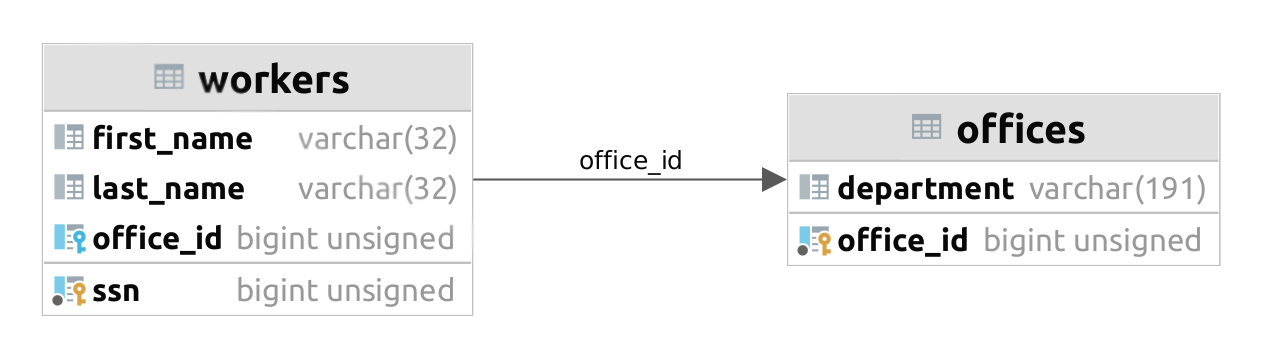
\includegraphics[width=1.15\textwidth]{MJ/assets/schema_office_example_cropped.svg.png}}
    \caption{von GORM aus Listing \ref{lst:tech:gorm:ex1} generiertes Datenbankmodell}
    \label{img:tech:gorm:schema:ex1}
\end{figure}

\newpage
\noindent
In der obigen Abbildung wird auch bereits das Standardverhalten von GORM ersichtlich. GORM hat den Go-Datentyp \mono{string}, der im \mono{Department} nicht genauer definiert wurde als \mono{varchar(191)} übersetzt. Um solche, eher weniger optimalen Abbildungen von Go auf das Datenbankmodell zu vermeiden, sollten Datentypen und Constraints immer explizit definiert werden um Konflikte zu vermeiden. 
Der Vollständigkeit halber befindet sich im Anhang (siehe Abschnitt \ref{sec:apdx:extendedcode}) der komplette Go-Code, der das in Abbildung \ref{img:tech:gorm:schema:ex1} veranschaulichte Datenbankmodell generiert.

\section{Gorilla}\label{sec:tech:gorilla}
Gorilla ist ein für die vorliegende Implementierung zum Einsatz kommendes Go-Toolkit, also eine Sammlung mehrerer Komponenten, mit der schnell und einfach Web Anwendungen entwickelt werden können (vgl. \cite{go:gorilla}). Gorilla beinhaltet Komponenten, unteranderem einen HTTP Multiplexer \mono{gorilla/mux}, der die eingehenden und ausgehenden HTTP-Anfragen an die richtigen Endpunkt-Handler weiterleitet. Eine weitere wichtige Komponente ist die Websocket-Bibliothek \mono{gorilla/websocket}, die ebenfalls für die vorliegende Implementierung zum Einsatz kommt. Schließlich wurde noch die Gorilla-Middleware Bibliothek \mono{gorilla/handlers}, in Kombination mit \textit{Meridian}, dem eigens für dieses Projekt entwickelte Middleware-Framework, eingesetzt.    

% \newpage
% \section{Technologien zur Dokumentation des Projektes}

% % \subsection{Swagger} 
% % (OpenAPI)

% \subsection{Textsatzsystem \LaTeX{}}
% Im Rahmen der vorliegenden Arbeit habe Ich mich umfassend mit dem Textsatzsystem \TeX{} und dessen erfolgreicher Erweiterung, \LaTeX{},  befasst. Auf der Suche nach einem vernünftigen System, um sauber und möglichst effizient, schöne Dokumente zu verfassen, experimentierte Ich mit einigen Systemen wie \textit{groff}, \textit{Markdown} und \textit{Con\TeX{}t}. Markdown zu wenige Features (ohnehin nicht dazu gedacht),  (Ablehnung der Profit und Consumer-orientierten Microsoft Philiosophie sowie zu kompliziert zu Verwenden)\\
% MS Word vs TeX: WYSIWYG vs WYSIWYAF (https://de.wikipedia.org/wiki/WYSIWYG)\\
% dokumentationsprojekt-struktur\\
% verwendete environments um text zu formatieren bzw. grafiken zu generieren\\
